\documentclass{beamer}
\mode<presentation>
\usepackage{amsmath,amssymb,mathtools}
\usepackage{textcomp}
\usepackage{gensymb}
\usepackage{adjustbox}
\usepackage{subcaption}
\usepackage{enumitem}
\usepackage{multicol}
\usepackage{listings}
\usepackage{url}
\usepackage{graphicx} % <-- needed for images
\def\UrlBreaks{\do\/\do-}

\usetheme{Boadilla}
\usecolortheme{lily}
\setbeamertemplate{footline}{
  \leavevmode%
  \hbox{%
  \begin{beamercolorbox}[wd=\paperwidth,ht=2ex,dp=1ex,right]{author in head/foot}%
    \insertframenumber{} / \inserttotalframenumber\hspace*{2ex}
  \end{beamercolorbox}}%
  \vskip0pt%
}
\setbeamertemplate{navigation symbols}{}

\lstset{
  frame=single,
  breaklines=true,
  columns=fullflexible,
  basicstyle=\ttfamily\tiny   % tiny font so code fits
}

\numberwithin{equation}{section}

% ---- your macros ----
\providecommand{\nCr}[2]{\,^{#1}C_{#2}}
\providecommand{\nPr}[2]{\,^{#1}P_{#2}}
\providecommand{\mbf}{\mathbf}
\providecommand{\pr}[1]{\ensuremath{\Pr\left(#1\right)}}
\providecommand{\qfunc}[1]{\ensuremath{Q\left(#1\right)}}
\providecommand{\sbrak}[1]{\ensuremath{{}\left[#1\right]}}
\providecommand{\lsbrak}[1]{\ensuremath{{}\left[#1\right.}}
\providecommand{\rsbrak}[1]{\ensuremath{\left.#1\right]}}
\providecommand{\brak}[1]{\ensuremath{\left(#1\right)}}
\providecommand{\lbrak}[1]{\ensuremath{\left(#1\right.}}
\providecommand{\rbrak}[1]{\ensuremath{\left.#1\right)}}
\providecommand{\cbrak}[1]{\ensuremath{\left\{#1\right\}}}
\providecommand{\lcbrak}[1]{\ensuremath{\left\{#1\right.}}
\providecommand{\rcbrak}[1]{\ensuremath{\left.#1\right\}}}
\theoremstyle{remark}
\newtheorem{rem}{Remark}
\newcommand{\sgn}{\mathop{\mathrm{sgn}}}
\providecommand{\abs}[1]{\left\vert#1\right\vert}
\providecommand{\res}[1]{\Res\displaylimits_{#1}}
\providecommand{\norm}[1]{\lVert#1\rVert}
\providecommand{\mtx}[1]{\mathbf{#1}}
\providecommand{\mean}[1]{E\left[ #1 \right]}
\providecommand{\fourier}{\overset{\mathcal{F}}{ \rightleftharpoons}}
\providecommand{\system}{\overset{\mathcal{H}}{ \longleftrightarrow}}
\providecommand{\dec}[2]{\ensuremath{\overset{#1}{\underset{#2}{\gtrless}}}}
\newcommand{\myvec}[1]{\ensuremath{\begin{pmatrix}#1\end{pmatrix}}}
\newcommand{\mydet}[1]{\ensuremath{\begin{vmatrix}#1\end{vmatrix}}}

\newenvironment{amatrix}[1]{%
  \left(\begin{array}{@{}*{#1}{c}|*{#1}{c}@{}}
}{%
  \end{array}\right)
}

\newcommand{\myaugvec}[2]{\ensuremath{\begin{amatrix}{#1}#2\end{amatrix}}}
\let\vec\mathbf
% ---------------------

\title{Matgeo Presentation - Problem 5.5.8}
\author{ee25btech11056 - Suraj.N}

\begin{document}

\begin{frame}
  \titlepage
\end{frame}

\begin{frame}{Problem Statement}

If 
\[
\vec{A} = \myvec{1 & 1 & 1 \\ 0 & 1 & 3 \\ 1 & -2 & 1}
\]
find $\vec{A}^{-1}$. Hence, solve the system of equations
\[
x+y+z=6,\quad y+3z=11,\quad x-2y+z=0.
\]
\end{frame}

\begin{frame}{Data}

\begin{table}[h!]
  \centering
  \begin{table}[h!]
    \centering
    \begin{tabular}{|c|c|}
        \hline
        Point & Coordinates \\
        \hline
	    $A$ & $\myvec{1\\-1}$ \\
	    $B$ & $\myvec{-4\\2k}$ \\
	    $C$ & $\myvec{-k\\-5}$ \\
        \hline
    \end{tabular}
    \caption{Vertices of $\triangle ABC$ before substituting $k$}
    \label{tab:triangle_k}
\end{table}

  \caption*{Table : Matrices}
  \label{5.5.8}
\end{table}

\end{frame}

\begin{frame}{Solution}

Forming the augmented matrix,

\begin{align}
  \myaugvec{3}{1 & 1 & 1 & 1 & 0 & 0\\0 & 1 & 3 & 0 & 1 & 0\\1 & -2 & 1 & 0 & 0 & 1 }
\end{align}

Applying elementary row operations to find the inverse,

\begin{align}
\myaugvec{3}{1 & 1 & 1 & 1 & 0 & 0\\0 & 1 & 3 & 0 & 1 & 0\\1 & -2 & 1 & 0 & 0 & 1 }
\xleftrightarrow{\;R_3 \to R_3 - R_1}
\myaugvec{3}{1 & 1 & 1 & 1 & 0 & 0\\0 & 1 & 3 & 0 & 1 & 0\\0 & -3 & 0 & -1 & 0 & 1 }\\
\xleftrightarrow{\;R_3 \to R_3 + 3R_2}
\myaugvec{3}{1 & 1 & 1 & 1 & 0 & 0\\0 & 1 & 3 & 0 & 1 & 0\\0 & 0 & 9 & -1 & 3 & 1 }
\end{align}

\end{frame}

\begin{frame}{Solution}

\begin{align}
\myaugvec{3}{1 & 1 & 1 & 1 & 0 & 0\\0 & 1 & 3 & 0 & 1 & 0\\0 & 0 & 9 & -1 & 3 & 1 }
\xleftrightarrow{\;R_3 \to \tfrac{R_3}{9}}
\myaugvec{3}{1 & 1 & 1 & 1 & 0 & 0\\0 & 1 & 3 & 0 & 1 & 0\\0 & 0 & 1 & -\tfrac{1}{9} & \tfrac{1}{3} & \tfrac{1}{9} }\\
\xleftrightarrow[\;R_1 \to R_1 - R_3\;]{\;R_2 \to R_2 - 3R_3}
\myaugvec{3}{1 & 1 & 0 & \tfrac{10}{9} & -\tfrac{1}{3} & -\tfrac{1}{9}\\0 & 1 & 0 & \tfrac{1}{3} & 0 & -\tfrac{1}{3}\\0 & 0 & 1 & -\tfrac{1}{9} & \tfrac{1}{3} & \tfrac{1}{9} }
\end{align}

\begin{align}
\myaugvec{3}{1 & 1 & 0 & \tfrac{10}{9} & -\tfrac{1}{3} & -\tfrac{1}{9}\\0 & 1 & 0 & \tfrac{1}{3} & 0 & -\tfrac{1}{3}\\0 & 0 & 1 & -\tfrac{1}{9} & \tfrac{1}{3} & \tfrac{1}{9} }
\xleftrightarrow{\;R_1 \to R_1 - R_2}
\myaugvec{3}{1 & 0 & 0 & \tfrac{7}{9} & -\tfrac{1}{3} & \tfrac{2}{9}\\0 & 1 & 0 & \tfrac{1}{3} & 0 & -\tfrac{1}{3}\\0 & 0 & 1 & -\tfrac{1}{9} & \tfrac{1}{3} & \tfrac{1}{9} }
\end{align}

\end{frame}

\begin{frame}{Solution}

The right side part of the augmented matrix is $\vec{A}^{-1}$

\begin{align}
  \vec{A}^{-1} &= \myvec{\tfrac{7}{9} & -\tfrac{1}{3} & \tfrac{2}{9}\\\tfrac{1}{3} & 0 & -\tfrac{1}{3}\\-\tfrac{1}{9} & \tfrac{1}{3} & \tfrac{1}{9}}
\end{align}

The solution for the system of equations is :

\begin{align}
  \vec{A}\vec{x} &= \vec{b}\\
  \vec{x} &= \vec{A}^{-1}\vec{b}\\
  \myvec{x\\y\\z} &= \myvec{\tfrac{7}{9} & -\tfrac{1}{3} & \tfrac{2}{9}\\\tfrac{1}{3} & 0 & -\tfrac{1}{3}\\-\tfrac{1}{9} & \tfrac{1}{3} & \tfrac{1}{9}}\myvec{6\\11\\0}\\
  \myvec{x\\y\\z} &= \myvec{1\\2\\3}
\end{align}

\end{frame}

\begin{frame}{Solution}

Therefore the solution is :

\begin{align}
\myvec{x\\y\\z} &= \myvec{1\\2\\3}
\end{align}

\end{frame}

\begin{frame}{Plot}

\begin{figure}[h!]
  \centering
  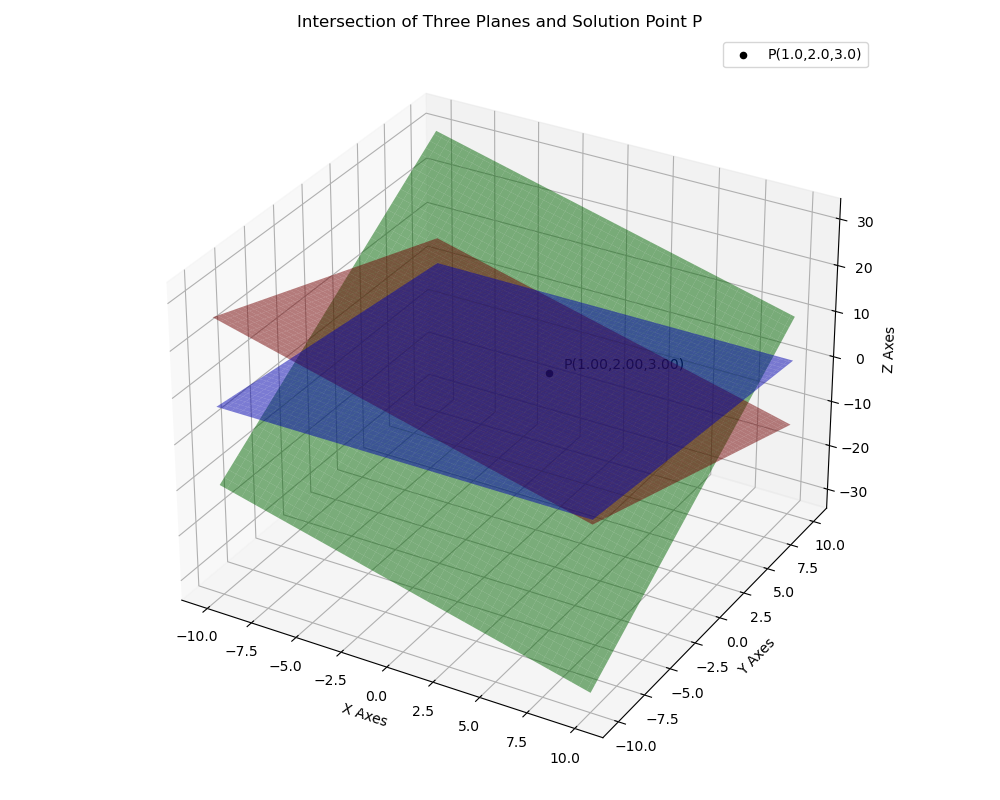
\includegraphics[width=0.7\columnwidth]{figs/solution.png} 
   \caption*{Fig : Planes}
  \label{Fig1}
\end{figure}

\end{frame}

\end{document}

